\documentclass[conference]{IEEEtran}
\IEEEoverridecommandlockouts

% Packages
\usepackage{cite}
\usepackage{amsmath,amssymb,amsfonts}
\usepackage{graphicx}
\usepackage{textcomp}
\usepackage{xcolor}
\usepackage{hyperref}
\usepackage{url}

\def\BibTeX{{\rm B\kern-.05em{\sc i\kern-.025em b}\kern-.08em
    T\kern-.1667em\lower.7ex\hbox{E}\kern-.125emX}}

\begin{document}

\title{Automated PCB Dataset Generation Pipeline for Segmentaion of Top Down PCB Images to Identify Components and Probing Areas of Interest}

\author{\IEEEauthorblockN{Zach Radlicz}
\IEEEauthorblockA{\textit{EE 5521 Final Project} \\
\textit{University of Minnesota}\\
Minneapolis, MN \\
radli009@umn.edu}
}

\maketitle

\begin{abstract}
This report covers the development of a dataset generation pipeline for rendered images of procedurally generated 3D models of PCBs for segmentation, and the training of a corresponding segmentation example model with Unet architecture. The generation pipeline relies on heavy GPU use for rendering as well as CPU use for preprocessing and creating 3D models. The pipeline is highly configurable through easily human readable YAML files and allows for significant tuning for different types of PCBs. Results show effective automatic dataset generation and successful machine learning model training.
\end{abstract}

\begin{IEEEkeywords}
PCB, segmentation, dataset generation, deep learning, U-Net, procedural generation
\end{IEEEkeywords}

\section{Introduction and Background}

PCBs are ubiquitous in the field of electronics and are the most common way for electrical systems to be put into production in consumer electronics and robotics. When it comes to hardware on PCBs it is much more difficult to debug and analyze than software. Debugging software has extremely well developed computational tools that are lacking in hardware. There is a need for machines to understand where areas of interest are on a PCB for probing and collecting data automatically, without human intervention.

Some PCB datasets exist that can be used for training vision models to detect areas of interest on PCBs, for example \cite{huang2015pcb}, which is a ~9000 image labeled dataset with bounding boxes for IC identification. Another example is \cite{keremberke2023pcb} which is a dataset for detecting defects on PCBs. As a segmentation example, this vision dataset exists as well \cite{pcbvision2023}. These are all valuable datasets for analyzing PCBs, but have significant shortcomings when it comes to accurately identifying probing areas of interest. The bounding boxes allow for IC identification, but not a precise location to actually place a probe. Defects are extremely valuable to be able to catch, but once again offer little to no spatial information about probe placement. Finally, the existing segmentation dataset is extremely valuable, however it only contains 53 images. This is not enough to train accurate segmentation models on, especially for a wide variety of PCBs that you may be likely to encounter.

The main reason that a huge segmentation dataset for PCBs doesn't exist is because PCBs can be incredibly dense and extremely varied in components, meaning obtaining accurate labels is incredibly time intensive. This report offers a potential solution by providing a highly configurable dataset generator to create any type of labelled PCB image programmatically.

\section{Methods}

\subsection{Architecture}

The architecture of the dataset generation system can be broken up into 5 distinct parts: Component Placement, PCB generation, Model Export/Import, Rendering, and Model Training. Each of these components is implemented using python scripts to automate functionality in KiCad, an open source EDA software and Blender with BlenderProc, a 3D modelling software. The entire application stack is containerized using Docker for deployment on HPC systems or other high compute systems. All configuration parameters for the generation pipeline are adjustable using three YAML files.

The development of this pipeline was significantly assisted by Claude Code, an AI-powered coding assistant based on Anthropic's Claude Sonnet 4.5 model \cite{claudecode2024}. Claude Code was used for implementing the modular architecture, debugging complex integration issues between KiCad and Blender, and optimizing the HPC deployment scripts. All of the code for this project can be found at \url{github.com/zradlicz/pcb-dataset-generator}.

% FIGURE PLACEHOLDER: Architecture Overview
\begin{figure}[htbp]
\centerline{\includegraphics[width=\columnwidth]{figures/architecture_overview.png}}
\caption{Overview of the PCB dataset generation pipeline architecture showing the five main components and their interactions.}
\label{fig:architecture}
\end{figure}

\subsection{Component Placement}

The component placement is driven by a procedural program based on Perlin noise to simulate realistic component placement on a PCB. Inspiration for this part of the process was taken from map generation techniques and city building procedural programs used in open world video games \cite{holmgard2016procedural}. Common PCB components were assembled into a library containing over 40 component types including resistors, capacitors, ICs of various pin counts, JST connectors, LEDs, diodes, and test points. Components are filtered based on their size, and larger components are placed closer to areas with high Perlin noise value. Once a large component is placed, very small components are more likely to be placed nearby to simulate decoupling capacitors commonly found on PCBs.

The placement algorithm uses an adaptive grid system with Perlin noise clustering and proper collision detection to ensure components don't overlap. Size-aware spacing is enforced, with typical boards containing around 148 components spread across small, medium, and large categories. A vignette effect with configurable strength is applied to prevent edge overcrowding, which would be unrealistic on actual PCBs. The configurable parameters for this step include Perlin noise octaves, persistence, lacunarity, number of small medium and large components, component type densities, vignette strength, and board dimensions. A full list can be found in the placement.yaml in Appendix A.

% FIGURE PLACEHOLDER: Component Placement
\begin{figure}[htbp]
\centerline{\includegraphics[width=\columnwidth]{figures/perlin_noise_placement.png}}
\caption{Visualization of Perlin noise-based component placement showing (a) Perlin noise map, (b) component density distribution, and (c) final component layout.}
\label{fig:placement}
\end{figure}

\subsection{PCB Generation}

In order to actually generate a PCB once the placement of the components is determined, open source EDA software KiCad is utilized. KiCad was chosen because it is free and open source, and also provides programmatic python access through its pcbnew package \cite{kicad2023}. This package includes PCB editing with trace drawing, component on board placement, file saving and download. KiCad importantly also provides the ability to add plugins that extend functionality. By using pcbnew, the component placement x and y values can be directly used, along with an overlap detection algorithm to arrange the components correctly. KiCad also maintains a vast library of 3D models and footprints that are connected to each component. It has a built in 3D model viewer.

To make the boards more realistic, a routing module generates copper traces connecting components. Random netlists are created including power, ground, and signal nets, with typically 30+ nets per board. Multiple routing algorithms are employed including straight traces, dogleg routing, and Manhattan-style routing to create varied and realistic trace patterns. All components are verified to load with their associated 3D models from KiCad's component libraries, which is critical for the rendering step. The soldermask layer is also properly configured, as this is essential for realistic visual appearance in the final renders.

% FIGURE PLACEHOLDER: PCB Generation Example
\begin{figure}[htbp]
\centerline{\includegraphics[width=\columnwidth]{figures/kicad_pcb_example.png}}
\caption{Example of a procedurally generated PCB in KiCad showing component placement, traces, and routing.}
\label{fig:pcb_generation}
\end{figure}

\subsection{Model Export/Import}

Since KiCad allows plugins, a convenient plugin was used for transferring the KiCad board file to Blender, which provides better rendering capabilities for realistic looking images. The package is called pcb2blender \cite{pcb2blender2023}. This plugin was added as a submodule in the GitHub repository to use as a bridge between KiCad and Blender.

A critical technical detail emerged during development: the export process uses KiCad's command-line tool (kicad-cli) rather than the Python API for VRML export. The GUI-based Python API export doesn't work in headless mode, which is required for HPC deployment. The command used is \texttt{kicad-cli pcb export vrml --units m --user-origin 0x0mm}, where the units must be meters (Blender interprets VRML as meters) and the origin must be set explicitly to prevent solder pad offset issues. This was a key learning from initial development attempts.

The pcb2blender plugin comes with two tools: an exporter from KiCad that converts the board to VRML format, and an importer for Blender that processes the VRML into Blender scenes with proper materials and object organization. Once the file is imported to Blender, it can be saved as a .blend file and additional rendering can be done on it at that point.

\subsection{Rendering}

Blender offers excellent rendering tools and allows programmatic python interaction, so it was a natural pick for this part of the process. Blender can also be extended with BlenderProc. BlenderProc makes Blender into a dataset creation tool that allows pixel level masking to be done automatically based on model attributes within Blender.

The segmentation strategy is material-based, relying on inspection of Mat4cad BSDF shader nodes that come from the pcb2blender import. The algorithm inspects each material's node tree, checking for the \texttt{mat\_base} property where a value of 2 indicates a metal surface. Objects with multiple materials are automatically split by material to enable per-face segmentation. The 3 classes chosen for this type of segmentation are: Class 0 (background), Class 1 (metal - including solder joints, component pins/leads, exposed copper, and test points), and Class 2 (non-metal - including component plastic/ceramic bodies and soldermask).

In development testing, the system successfully detected 755 metal objects and 145 non-metal objects across 30 component types. A known limitation is that the PCB substrate currently appears as all metal due to copper and soldermask being grouped together - future work could address this with texture-based splitting. Once the classes are defined, BlenderProc automatically creates segmentation maps including category\_id, material, instance, and name-based masks when rendering.

For the example dataset, the render images were created with a resolution of 1024x1024 pixels. This was chosen for generation timeline purposes and to balance detail with computational efficiency. The renderer configuration allows variation in camera location, lighting location, soldermask color, material filtering, etc. A full list can be found in render.yaml in Appendix A.

% FIGURE PLACEHOLDER: Rendering Examples
\begin{figure}[htbp]
\centerline{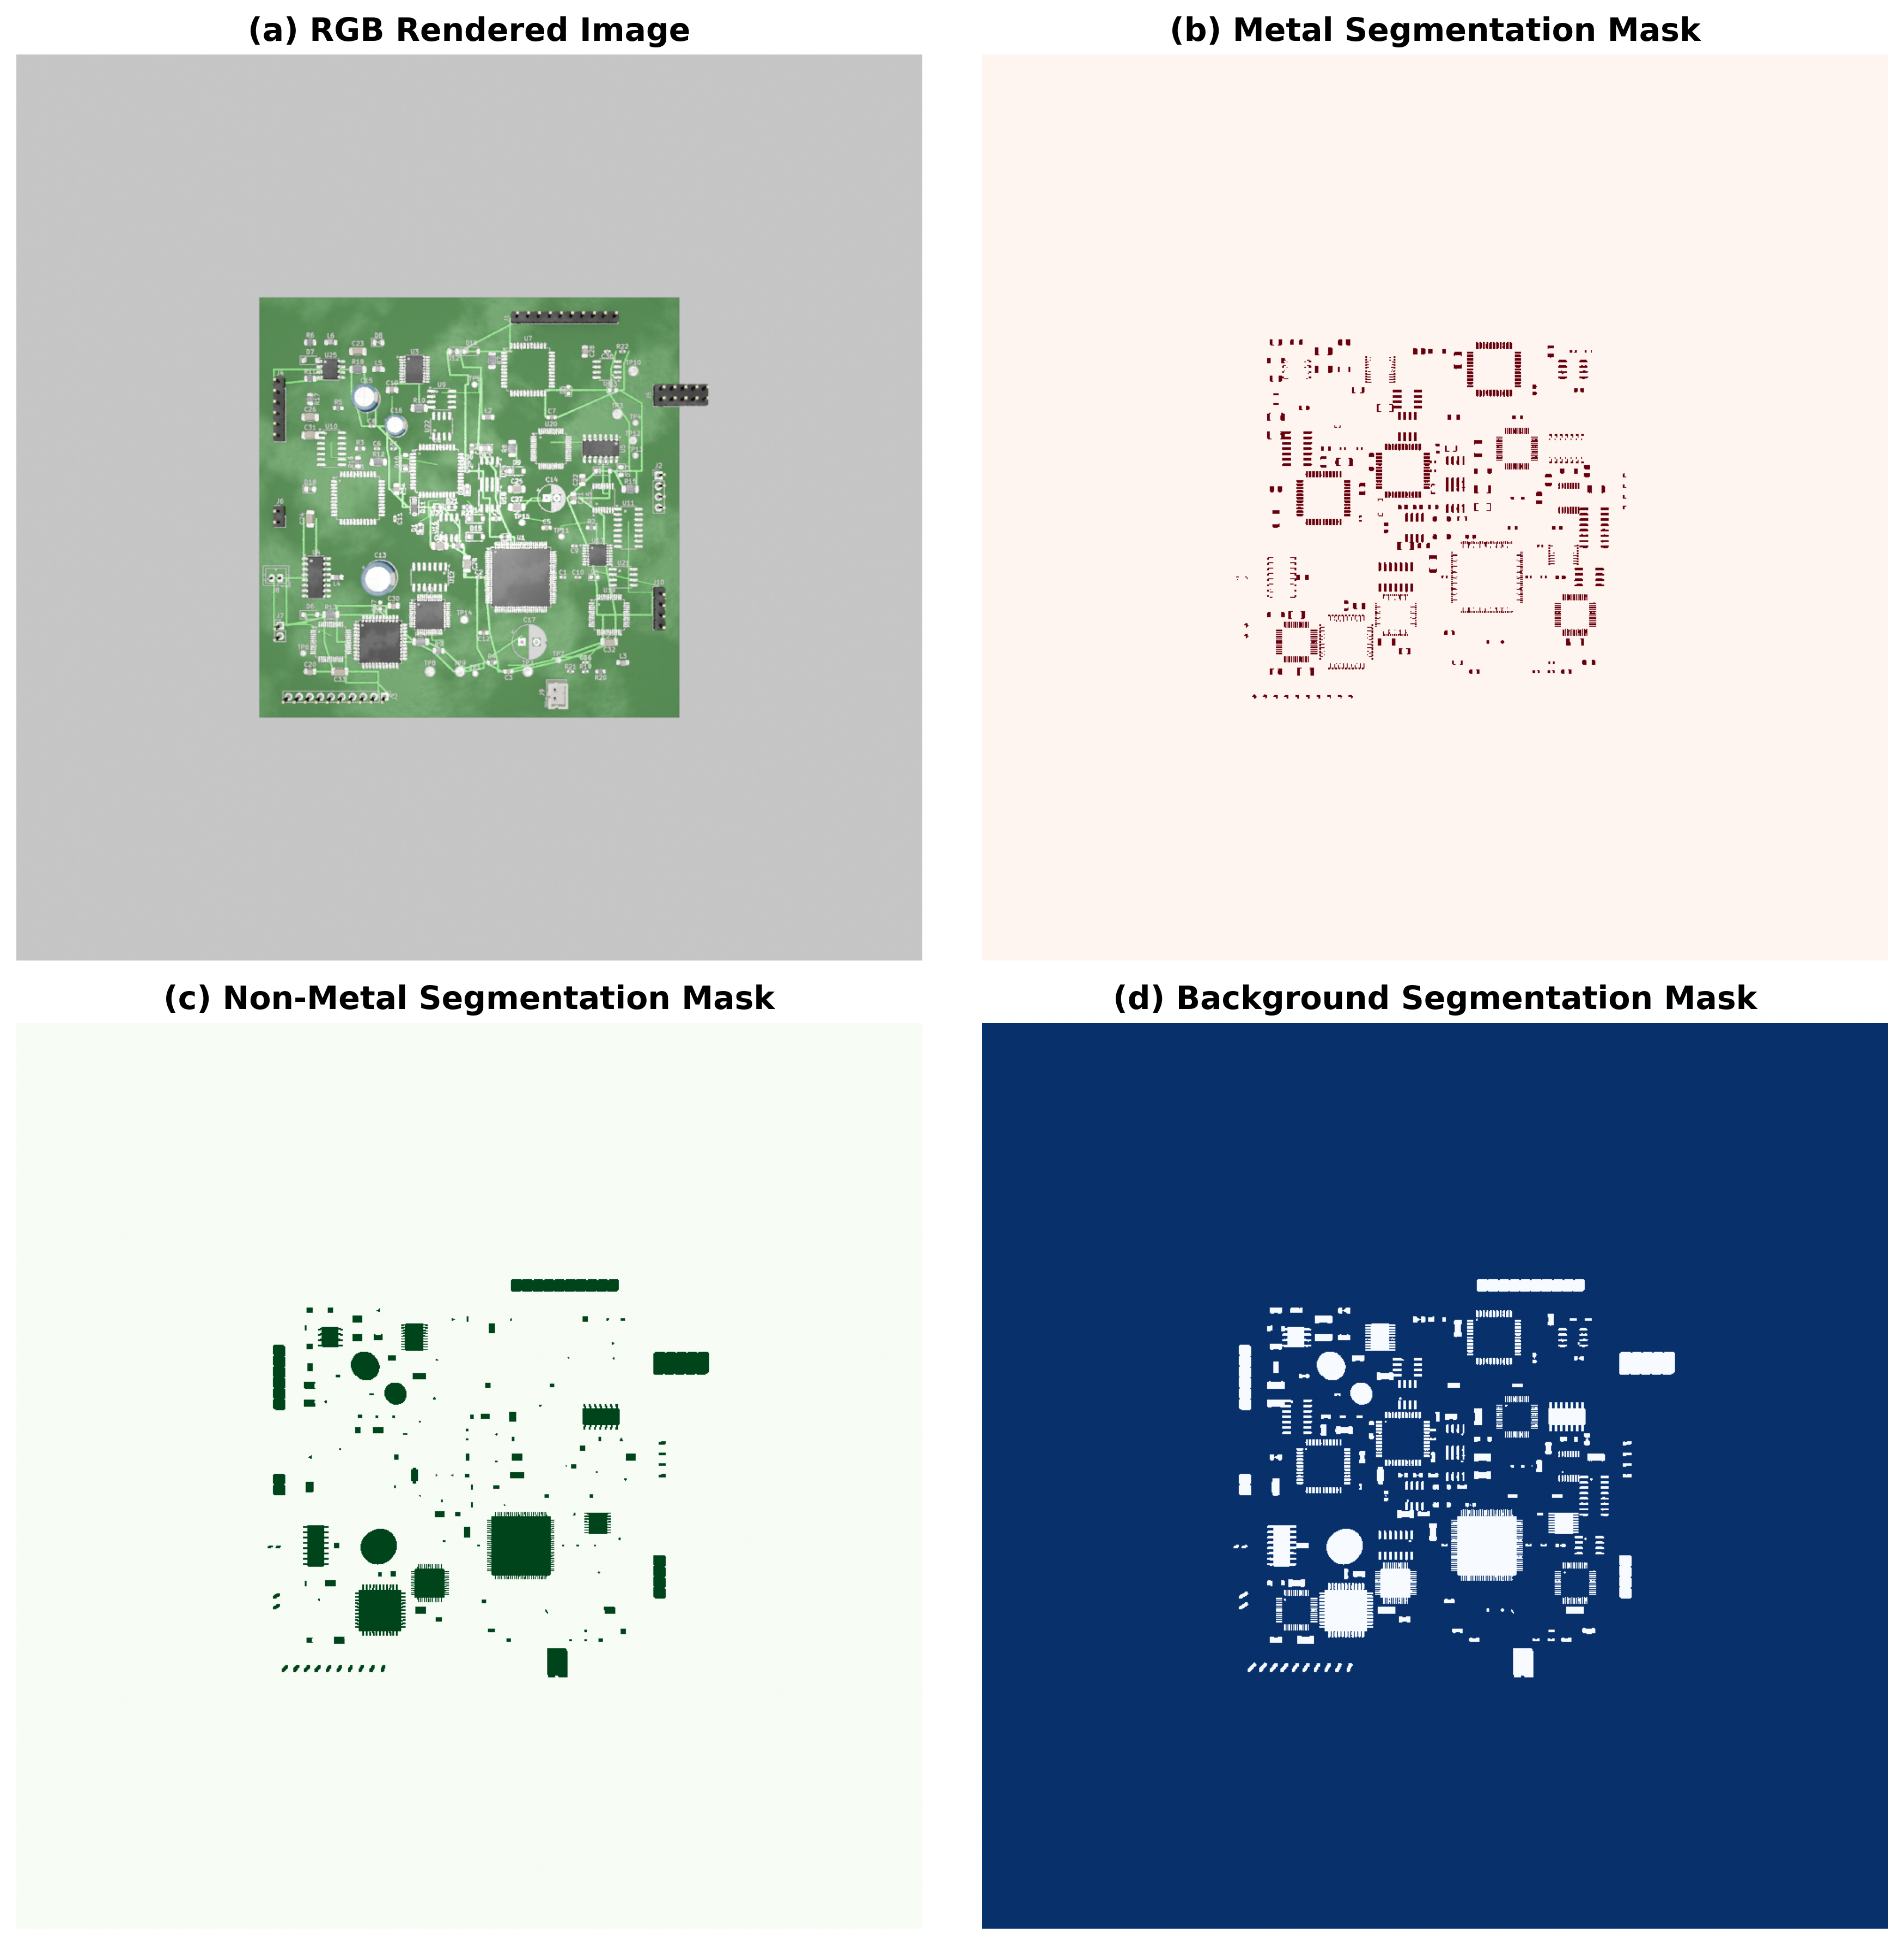
\includegraphics[width=\columnwidth]{figures/rendering_example.png}}
\caption{Example rendering output showing (a) RGB rendered image, (b) metal segmentation mask, (c) soldermask segmentation mask, and (d) other materials segmentation mask.}
\label{fig:rendering}
\end{figure}

\subsection{Model Training}

Once a dataset is generated, a basic U-Net segmentation model \cite{ronneberger2015unet} was trained to segment the images. PyTorch was chosen as a machine learning framework, and analysis was done in a Jupyter notebook using Google Colab for reproducibility by anyone. Significant preprocessing was done after the dataset generation. In order to train the model in a short amount of time on Google Colab, downsizing of the generated image resolution was employed. Random 256x256 crops of each photo were taken, in order to provide some stochasticity to where board boundaries were in the image. This was in order to prevent overtraining and the model learning to label only in the center of images. For the proposed application, a camera would be facing downwards on a PCB and the PCB may not necessarily be centered in frame. 256x256 also allowed for training the model without overtaking VRAM limitation on the 16GB GPU available on Google Colab. For the training portion of this report, a 70-30 split was chosen for training and validation data. CrossEntropyLoss was chosen as a loss function, as was Adam optimizer. This was copied from the U-Net segmentation model paper.

% FIGURE PLACEHOLDER: U-Net Architecture
\begin{figure}[htbp]
\centerline{\includegraphics[width=\columnwidth]{figures/unet_architecture.png}}
\caption{U-Net architecture used for PCB segmentation with input size 256x256 and 3 output classes.}
\label{fig:unet}
\end{figure}

\subsection{Infrastructure}

The compute required to run the dataset generation pipeline is significant and not feasible on consumer level hardware due to the high number of rendering tasks. For this reason, the entire pipeline was containerized using Docker. Docker allows for deployment on any type of system. The Docker image was built with KiCad 8.0, Blender 4.2, BlenderProc, and all Python dependencies, then pushed to Docker Hub for easy deployment. For HPC execution, the Docker image is converted to Apptainer/Singularity format, which is the standard container runtime for HPC clusters.

For the example generated dataset in this report, Minnesota Supercomputing Institute (MSI) was leveraged. SLURM, the job scheduling system used by MSI, allows for scripting and job arrays, so scripts defining the necessary compute resources are provided in the repository. The pipeline is split into two stages for optimal resource utilization.

The first stage runs CPU-intensive tasks on the msismall partition with 16 CPUs and 32GB RAM per task. This includes component placement, PCB generation, VRML export, and Blender import - all the steps needed to create a .blend file. These tasks run in parallel using SLURM array jobs. The second stage runs GPU-intensive rendering on the msigpu partition. Once a directory of .blend files is available, rendering is performed with GPU acceleration. For the example generation, A100 GPUs were requested, though the system supports flexible GPU selection including H100, A40, L40S, and V100 options.

This split approach dramatically improves efficiency by running hundreds of CPU jobs in parallel on cheaper CPU nodes, then using expensive GPU time only for the fast rendering step. Resource requirements per sample are approximately 30-60 minutes of CPU time and 1.5 hours of GPU time. The system has been proven at scale, generating 1000 samples in production.

\section{Results}

The results of the data generation pipeline and example model training were mixed. As a demonstration of the capabilities, 1000 images were generated using MSI as a compute engine. The split generation schema was used to isolate CPU and GPU intensive tasks. Out of 1000 generated images, 695 completed the rendering process. After integrity validation to filter corrupted HDF5 files, 689 usable samples remained - a 31\% loss rate from the initial target. The corruption was due to BlenderProc rendering failures during the generation pipeline, which is an area for improvement in future work.

The 689 valid samples were split into training (482 samples, 70\%), validation (137 samples, 20\%), and test (70 samples, 10\%) sets. The U-Net model has 31 million parameters and was trained for 50 epochs using CrossEntropyLoss and Adam optimizer with a learning rate of 1e-4. Training was performed on Google Colab with a Tesla T4 GPU and took approximately 10 minutes total. The best model was selected from epoch 6 based on validation loss (0.0939).

On the test set, overall pixel accuracy of 98.5\% was achieved. However, per-class accuracy varied significantly: 99.88\% for Class 0 (Background), 58.90\% for Class 1 (metal), and 85.81\% for Class 2 (non-metal/plastic). The mean IoU across classes was 77.87\% and mean Dice coefficient was 86.08\%. These metrics are assessed on generated images from the generation pipeline, where the model performs well because the domain matches the training distribution.

% FIGURE PLACEHOLDER: Training Results
\begin{figure}[htbp]
\centerline{\includegraphics[width=\columnwidth]{figures/training_curves.png}}
\caption{Training and validation loss curves over 6 epochs.}
\label{fig:training}
\end{figure}

% FIGURE PLACEHOLDER: Per-Class Accuracy
\begin{figure}[htbp]
\centerline{\includegraphics[width=\columnwidth]{figures/class_accuracy.png}}
\caption{Per-class pixel accuracy showing performance across background, metal, and plastic classes.}
\label{fig:accuracy}
\end{figure}

On real world images, the results can only be analyzed qualitatively. The results are not good, as the model failed to recognize metal in almost all cases except in a specific case where the lighting made the copper traces look significantly more white colored than copper colored.

% FIGURE PLACEHOLDER: Real World Results
\begin{figure}[htbp]
\centerline{\includegraphics[width=\columnwidth]{figures/real_world_comparison.png}}
\caption{Comparison of model performance on (a) generated images vs (b) real-world PCB images, showing the sim-to-real gap.}
\label{fig:realworld}
\end{figure}

\section{Discussion}

The results are expected for this type of system. Since the generation pipeline was not tuned at all for realism, this project was more of a proof of concept that a fully automated generated dataset could be used to train a machine learning model that has use in the real world. I think the concept of this is extremely promising even if the results were not great, as some tuning of the pipeline could drastically improve the results.

\section{Domain Randomization Implementation}

To address the sim-to-real gap identified in the initial results, comprehensive domain randomization has been implemented across both the rendering and placement pipelines. This randomization provides the variability needed to improve model generalization to real-world PCBs.

\subsection{Rendering Domain Randomization}

The rendering pipeline now supports stochastic variation of the following parameters for each generated sample:

\textbf{Lighting Randomization:} Sun light intensity varies uniformly between 1.5-3.0 (previously fixed at 2.0), sun rotation varies across all three axes with ranges of $\pm$0.3 radians for pitch/yaw and 0-6.28 radians for full rotation around the vertical axis, and fill light intensities vary between 0.3-0.9 (previously fixed at 0.6). This simulates different times of day, lighting conditions, and workshop environments.

\textbf{Camera Randomization:} Camera position offsets of $\pm$2cm in horizontal directions add perspective variation while maintaining top-down orientation. Camera rotation offsets of $\pm$0.1 radians ($\pm$5.7°) for pitch and roll, and $\pm$0.2 radians ($\pm$11.5°) for yaw simulate realistic camera mounting variations and hand-held capture scenarios.

\textbf{Background Randomization:} Six background color options ranging from white (0.95, 0.95, 0.95) to dark surfaces (0.3, 0.3, 0.35) simulate different work surfaces including clean benches, wood desks, and dark mats.

\textbf{Soldermask Color Randomization:} Seven common PCB soldermask colors (green, blue, red, black, white, yellow, and purple) are randomly selected with appropriate metallic and roughness properties. This addresses the unrealistic uniformity of the original dataset where all boards were green.

\subsection{Placement Domain Randomization}

The component placement pipeline now supports randomization of procedural generation parameters:

\textbf{Perlin Noise Randomization:} Scale varies between 20.0-40.0 (affecting noise smoothness), octaves vary between 3-5 (detail levels), persistence varies between 0.4-0.6 (amplitude decay), and lacunarity varies between 1.8-2.2 (frequency increase). This creates diverse organic clustering patterns.

\textbf{Component and Board Variation:} Vignette strength varies between 0.5-0.9 for edge density falloff, component counts vary by $\pm$20\% from baseline values, and board dimensions vary between 80-120mm with options for rectangular or square shapes.

All randomization parameters are configurable via YAML files (render.yaml and placement.yaml) with a master enable/disable switch. When enabled, each generated sample receives a unique combination of parameters sampled from the specified ranges, creating a diverse dataset that better represents real-world variability.

\section{Future Development and Improvements}

While domain randomization has been implemented, additional improvements can further enhance the pipeline. Higher resolution renders (2048x2048 or higher) would provide better detail for extremely small components. Improvements to the generation stability would help address the 31\% sample loss rate from rendering failures and HDF5 corruption.

The sim-to-real gap, while reduced through domain randomization, can be further addressed through advanced techniques. Future proposals include using state-of-the-art vision language models (VLMs) to translate image 'style' to match a user's particular PCB characteristics and camera setup. Another possibility is using a VLM for semi-supervised labeling of a small number of real user PCB images, then fine-tuning the existing model with this real-world data. Additional physical realism could be added through component aging effects, surface defects, dust, and reflections. HDRI environment maps could replace simple background colors to provide photorealistic lighting and reflections.

\section{Conclusion}

This work presents an automated pipeline for generating synthetic PCB datasets with pixel-level segmentation labels. The system successfully generates realistic PCB layouts using Perlin noise-based procedural generation and produces high-quality rendered images with corresponding segmentation masks. Domain randomization has been implemented across both rendering and placement pipelines to address the sim-to-real gap, providing stochastic variation in lighting, camera angles, soldermask colors, background surfaces, and procedural generation parameters. While the trained U-Net model achieves high accuracy on synthetic data (98.5\% overall pixel accuracy), continued work on photorealism and semi-supervised learning with real-world data will further improve deployment performance. Future work will focus on leveraging vision language models for style transfer and semi-supervised labeling, and incorporating additional physical realism effects. The open-source nature of this pipeline, with comprehensive domain randomization capabilities, provides a foundation for the research community to develop more robust PCB analysis tools.

\begin{thebibliography}{00}
\bibitem{huang2015pcb} W. Huang and P. Wei, ``A PCB Dataset for Defects Detection and Classification,'' \textit{IEEE International Conference on Advanced Video and Signal Based Surveillance (AVSS)}, 2015. Available: https://ieeexplore.ieee.org/document/7153209

\bibitem{keremberke2023pcb} ``PCB Defect Segmentation Dataset,'' Hugging Face, 2023. Available: https://huggingface.co/datasets/keremberke/pcb-defect-segmentation

\bibitem{pcbvision2023} ``PCBVision: Segmentation Dataset for PCBs,'' GitHub, 2023. Available: https://github.com/hifexplo/PCBVision

\bibitem{claudecode2024} ``Claude Code,'' Anthropic, 2024. Available: https://claude.com/claude-code

\bibitem{holmgard2016procedural} C. Holmgård et al., ``Procedural Content Generation in Games,'' \textit{arXiv preprint arXiv:1610.03525}, 2016.

\bibitem{kicad2023} ``KiCad Python API Documentation,'' KiCad Development Team, 2023. Available: https://dev-docs.kicad.org/en/apis-and-binding/pcbnew/index.html

\bibitem{pcb2blender2023} ``pcb2blender: KiCad to Blender Exporter,'' GitHub, 2023. Available: https://github.com/30350n/pcb2blender

\bibitem{ronneberger2015unet} O. Ronneberger, P. Fischer, and T. Brox, ``U-Net: Convolutional Networks for Biomedical Image Segmentation,'' \textit{arXiv preprint arXiv:1505.04597}, 2015.

\end{thebibliography}

\appendix
\section{Configuration Files}

The complete YAML configuration files (placement.yaml, render.yaml, and pipeline.yaml) are available in the project repository at \url{github.com/zradlicz/pcb-dataset-generator}.

\end{document}
